\documentclass[12pt,a4paper,twoside]{book}

%Nastaví kódování na UTF8
\usepackage[utf8]{inputenc}

%Nastavuje velikost vertikální mezery mezi odstavci
\setlength{\parskip}{1ex plus 0.5ex minus 0.2ex}

\usepackage[cc]{titlepic}
\usepackage{graphicx}
\usepackage{fancyhdr}
\pagestyle{fancy}
\renewcommand{\footrulewidth}{0.4pt}
\fancyfoot[CO,CE]{www.zonglovani.info}
\fancyfoot[RO, LE] {\thepage}

\usepackage{wrapfig}
\usepackage{floatflt}

\parindent=2.2em
\usepackage[czech]{babel}
\usepackage{indentfirst}

% vypnutí číslování nadpisů v textu
%\setcounter{secnumdepth}{-1}
\begin{document}
\renewcommand{\arraystretch}{1.1}
\setlength{\parindent}{0pt}

\title{Žonglérův slabikář}
\author{Petr Kletečka}
\date{}
\titlepic{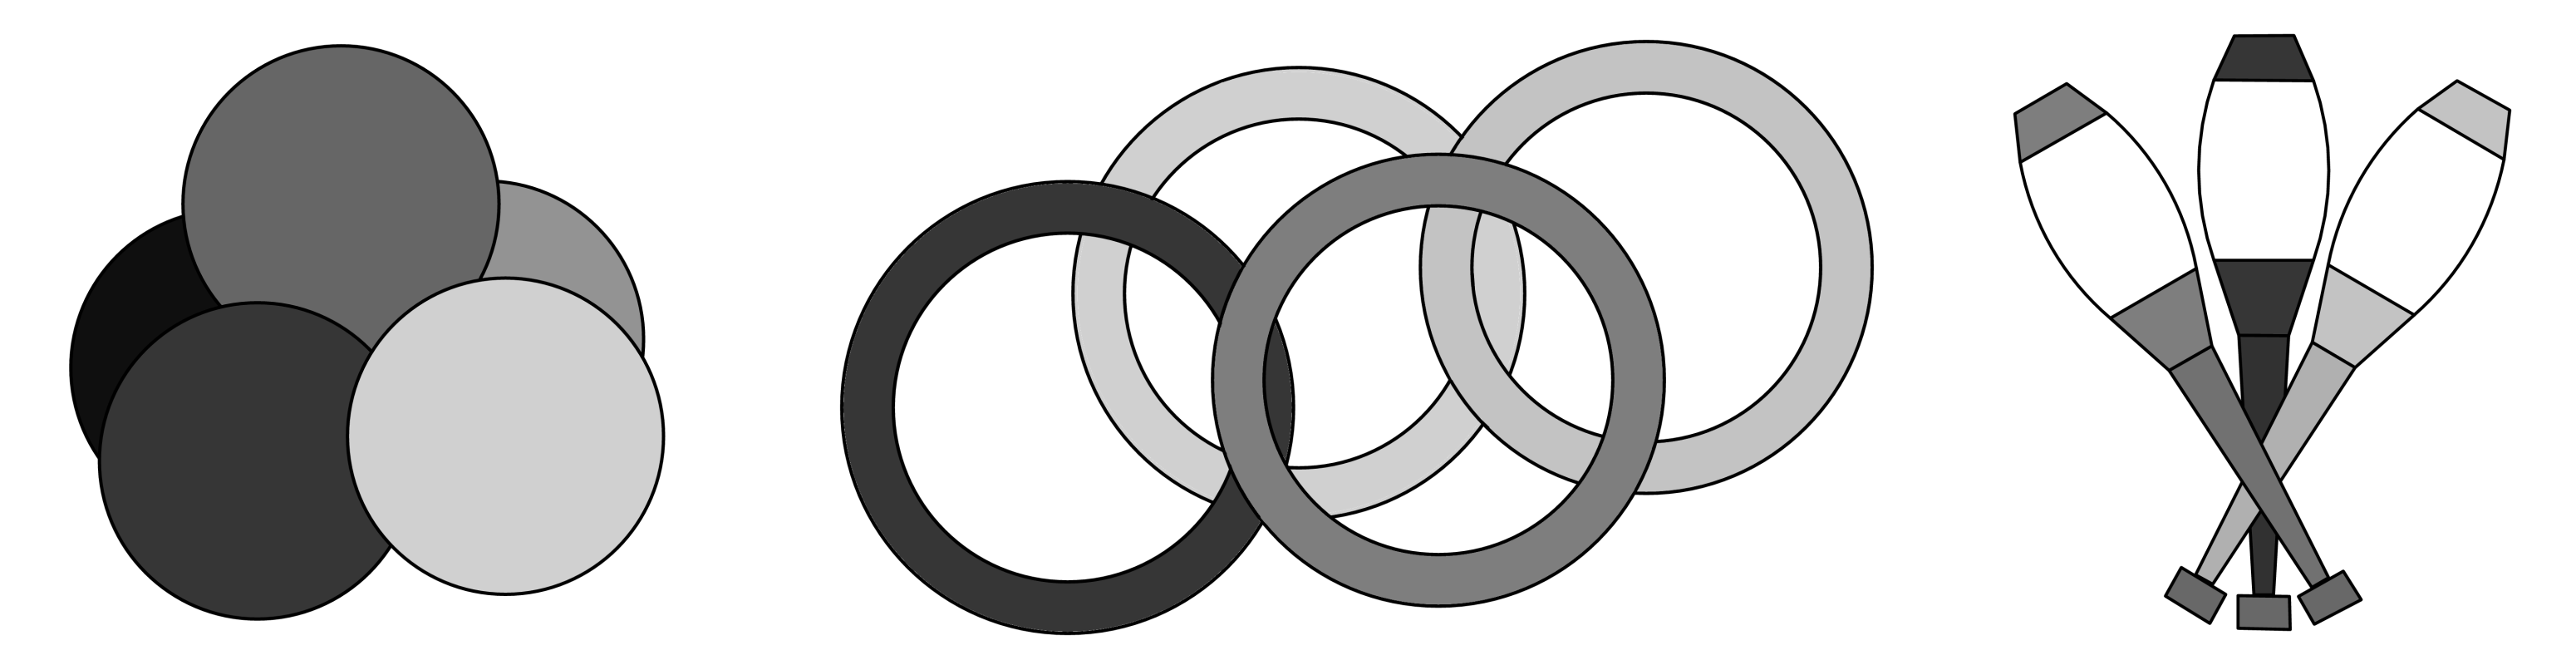
\includegraphics[width=\textwidth]{titleimg.png}}
\maketitle
\setcounter{tocdepth}{1}
\tableofcontents

\chapter{Tři míčky}

\include{tri-micky}

\chapter{Čtyři míčky}

\include{ctyri-micky}

\chapter{Pět míčků}

\include{pet-micku}

\end{document}
